\documentclass[a4paper,english,11pt,twoside]{article}
\usepackage[utf8]{inputenc}
\usepackage[T1]{fontenc}
\usepackage[english]{babel}
\usepackage{epsfig}
\usepackage{graphicx}
\usepackage{amsmath}
\usepackage{pstricks}
\usepackage{subcaption}
\usepackage{booktabs}
\usepackage{float}
\usepackage{gensymb}
\usepackage{preamble}
\usepackage{movie15}
\restylefloat{table}
\renewcommand{\arraystretch}{1.5}
 \newcommand{\tab}{\hspace*{2em}}


\date{\today}
\title{Mandatory Assignment 1}
\author{Jørgen D. Tyvand}

\begin{document}
\maketitle
\newpage

\section*{1)}

\section*{2)}
For both the LES and RANS models, we start from the Navier-Stokes equations for incompressible flow:\\
\\
$\nabla\cdot (\rho\vec{u}) = 0$\\
\\
$\pdi{(\rho u)}{t} + \nabla\cdot(\rho u \vec{u}) = -\pdi{p}{x} + \mu\nabla^2u$\\
\\
$\pdi{(\rho v)}{t} + \nabla\cdot(\rho v \vec{u}) = -\pdi{p}{y} + \mu\nabla^2v$\\
\\
Lengthy derivations of the LES and RANS equations will not be given, but a short explanation of each will give the general process.\\
\\
For Large Eddy Simulation (LES), we use spatial filtering to separate varying sizes of eddies. A cutoff width $\Delta$ is introduced, for which information about eddies smaller than the given width will be ignored/destroyed. A spatial filtering using a filter finction $G(\vec{x},\vec{x}', \Delta)$ is introduced, giving in the following form (3.84 in the book):\\
\\
$\ol\phi(\vec{x},t) \equiv \displaystyle\int\limits_{-\infty}^\infty\int\limits_{-\infty}^\infty\int\limits_{-\infty}^\infty\, G(\vec{x},\vec{x}', \Delta)\phi(\vec{x}', t)\mathrm dx_1'\mathrm dx_2'\mathrm dx_3'$\\
\\
where $\ol\phi(\vec{x},t)$ and $\phi(\vec{x}, t)$ are the filtered and unfiltered functions respectively. The filter function $G(\vec{x},\vec{x}', \Delta)$ can be given in several ways, but the one used in finite volume implementations is the top-hat/box filter function\\
\\
$
 G(\vec{x},\vec{x}', \Delta) = 
  \begin{cases} 
   \frac{1}{\Delta^3} & \abs{\vec{x} - \vec{x}'} \leq \Delta / 2 \\
   0       & \abs{\vec{x} - \vec{x}'} > \Delta / 2
  \end{cases}
$\\
\\
Using this filtering on the Navier-Stokes equations, we get the LES momentum equations (the intermediate step from 3.88a-c to 3.89a-c in the book for rewriting the term $\nabla\cdot(\rho\ol{\phi\vec{u}})$ is not shown):\\
\\
$\pdi{(\rho \ol{u})}{t} + \nabla\cdot(\rho \ol{u}\, \vec{\ol{u}}) = -\pdi{\ol{p}}{x} + \mu\nabla^2\ol{u} - (\nabla\cdot(\rho \ol{u\vec{u}}) - \nabla\cdot(\rho \ol{u}\, \vec{\ol{u}}))$\\
\\
$\pdi{(\rho \ol{v})}{t} + \nabla\cdot(\rho \ol{v}\, \vec{\ol{u}}) = -\pdi{\ol{p}}{y} + \mu\nabla^2\ol{v} - (\nabla\cdot(\rho \ol{v\vec{u}}) - \nabla\cdot(\rho \ol{v}\, \vec{\ol{u}}))$\\
\\
The boundary conditions for the LES problem is as following:\\
\\
Uniform velocity of 10 m/s in the x-direction at the inlet\\
Zero velocity gradient at the walls and outlet\\
Zero pressure gradient at the walls and inlet\\
A uniform value of 0 for the pressure at the outlet\\
\\
For the simulations i have used 2 different mesh refinements, one with 10x20 cells for the inlet and outlet boxes and 100x20 for the center boxes, as well as a doubled mesh of 20x40 and 200x40 boxes. The case files were originally copied from the PitzDaily case for incompressible flow with PISO, and edited from there. For the convection term i have tested different upwind schemes, and landed on filteredLinear. An upwind scheme will include more information from upwind cells, and therefore (hopefully) give a more correct and stable calculation. I have tested the following 4 schemes for the coarsest mesh:\\
\\
Non-upwind linear (as found in the unaltered PitzDaily files)\\
upwind\\
linearUpwind\\
filteredLinear\\
\\
The following four movie files shows a simulation of these four schemes for 0.5 seconds on the 100 mesh:\\
\begin{figure}[h!]
	\includemovie[poster,]{4cm}{4cm}{animation_piso_10.mp4}
\end{figure}

The filteredLinear scheme has also been used for the 200 mesh, as well as a even finer mesh of 250x50 central boxes. As we can see from the following videos, the solutions are mot mesh independent.\\
\\
I also found that the solver crashed if i used a too fine mesh with a too coarse time step. In the final calculations i have used timesteps of $1.0*10^{-5}$, but with a timestep of $1.0*10^{-4}$ the Courant number grew to between 1.5 and 2, at which the calculations crashed. This implies grid sensitivity with respect to grid size and time step size.
\section*{3)}
For the RANS models i have chosen to use the simpleFoam solver for the $k-\epsilon$ and $k-\omega$ models. The general RANS equations are as follows:\\
\\
Here the overline marks the mean terms, and the marked terms are the fluctuation terms.\\
\\
For the $k-\epsilon$ model, I have used the value for k that was used in the PitzDaily case. This is because the inlet velocity is the same, and i have assumed that a similar turbulence intensity is appropriate. Analyzing the value for $\epsilon$ in the PitzDaily case, i found that they have used a value of 0.1 times the inlet opening for the turbulent length scale. I have adjusted my value for $\epsilon$ using the same ratio.\\
\\
There are two additional equations to be solved for the $k-\epsilon$ model:\\
\\
$\pdi{\rho k}{t} + \nabla\cdot(\rho k \vec{u}) = \frac{\mu_t}{\sigma_k}\nabla^2k + 2\mu_t S_{ij}\cdot S_{ij} - \rho\epsilon$\\
\\
$\pdi{\rho \epsilon}{t} + \nabla\cdot(\rho \epsilon \vec{u}) = \frac{\mu_t}{\sigma_{\epsilon}}\nabla^2\epsilon + C_{1\epsilon}\frac{\epsilon}{k}2\mu_t S_{ij}\cdot S_{ij} - C_{2\epsilon}\rho\frac{\epsilon^2}{k}$\\
\\
Here, $S_{ij}$ are the components of the mean of the rate of deformation. The constants have the following given values (found both in the book and in other sources):\\
\\
$\mu_t = \rho C_{\mu}\frac{k^2}{\epsilon}\tab C_{\mu} = 0.09\tab\sigma_k = 1.00\tab\sigma_{\epsilon} = 1.30\tab C_{1\epsilon} = 1.44\tab C_{2\epsilon} = 1.92$
\\

Running the $k-\epsilon$ case, i have found the following converged solutions for the flow, using the 100 and 200 meshes respectively:\\
\\
The following figures show the mean velocity for the two mesh sizes:\\
\begin{figure}[h!]
	\begin{subfigure}{0.5\textwidth}
		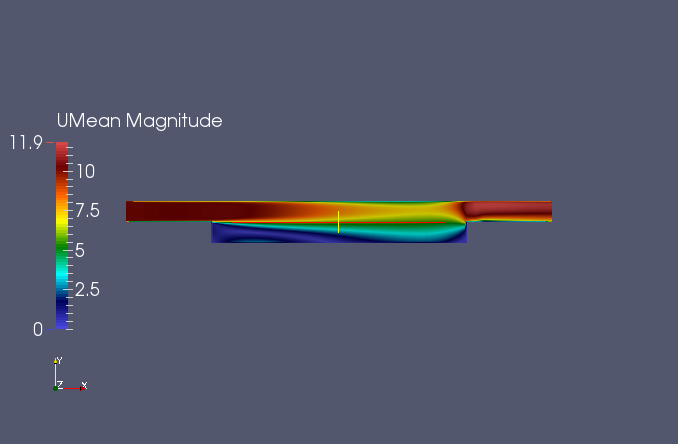
\includegraphics[width=0.95\linewidth]{simple_ke_10_mean_u.png}
	\end{subfigure}
	\begin{subfigure}{0.5\textwidth}
		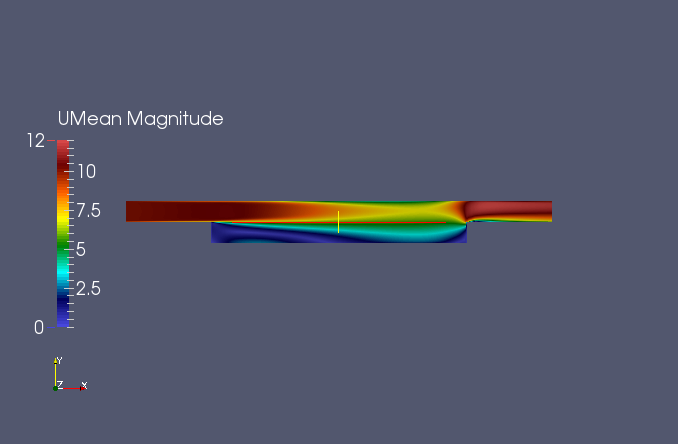
\includegraphics[width=0.95\linewidth]{simple_ke_20_mean_u.png}
	\end{subfigure}
\end{figure}
\\
And finally we have the mean kinematic energy:\\
\begin{figure}[h!]
	\begin{subfigure}{0.5\textwidth}
		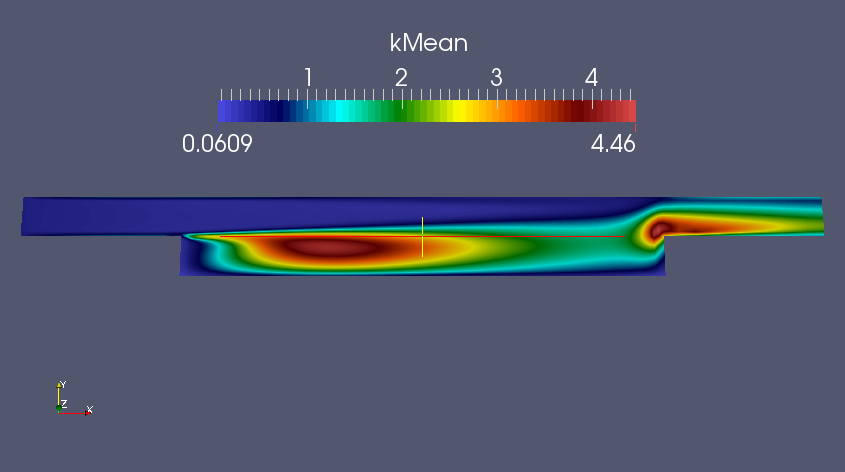
\includegraphics[width=0.95\linewidth]{simple_ke_10_mean_k.png}
	\end{subfigure}
	\begin{subfigure}{0.5\textwidth}
		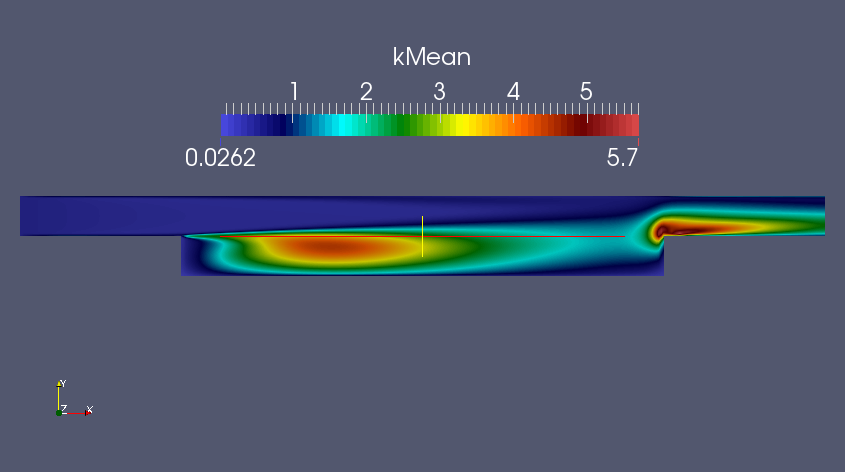
\includegraphics[width=0.95\linewidth]{simple_ke_20_mean_k.png}
	\end{subfigure}
\end{figure}
We see that there is virtually no difference between the two cases, so there is little or no mesh sensitivity using simpleFoam for this RANS problem.\\
\\
For the $k-\omega$ model, i have used the fact that $\omega = \frac{\epsilon}{k}$, and used the values from the $k-\epsilon$ problem to calculate $\omega$. We have two additional equations in this model as well:\\
\\
$\pdi{\rho k}{t} + \nabla\cdot(\rho k \vec{u}) = (\mu + \frac{\mu_t}{\sigma_k})\nabla^2k + P_k - \beta^*\rho k\omega\tab P_k = \left(2\mu_t S_{ij}\cdot S_{ij} - \frac{2}{3}\rho k\pdi{U_i}{x_j}\delta_{ij}\right)$\\
\\
$\pdi{\rho \omega}{t} + \nabla\cdot(\rho \omega \vec{u}) = (\mu + \frac{\mu_t}{\sigma_{\omega}})\nabla^2\omega + \gamma_i\left(2\rho S_{ij}\cdot S_{ij} - \frac{2}{3}\rho \omega\pdi{U_i}{x_j}\delta_{ij}\right) - \beta_1\rho\omega^2$\\
\\
With constants\\
\\
$\sigma_k = 2.0\tab\sigma_{\omega} = 2.0\tab\gamma_1 = 0.553\tab\beta_1 = 0.075\tab\beta^* = 0.09$\\
\\
Running simpleFoam, we get the following plots for the converged values of the mean velocity for the 100 and 200 meshes:\\
\begin{figure}[h!]
	\begin{subfigure}{0.5\textwidth}
		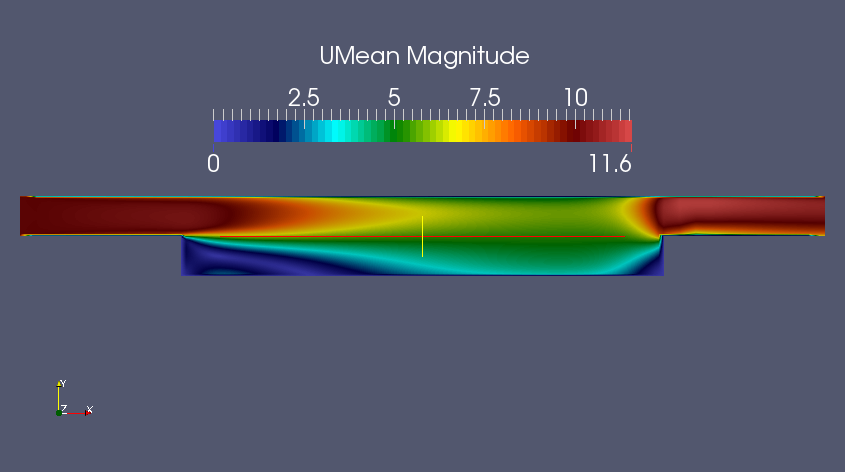
\includegraphics[width=0.95\linewidth]{simple_ko_10_mean_u.png}
	\end{subfigure}
	\begin{subfigure}{0.5\textwidth}
		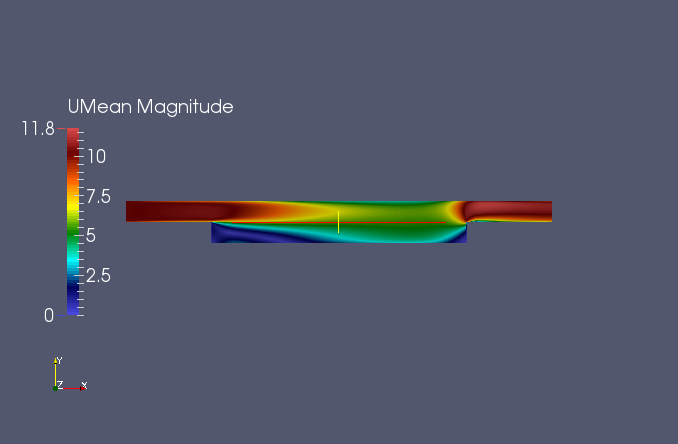
\includegraphics[width=0.95\linewidth]{simple_ko_20_mean_u.png}
	\end{subfigure}
\end{figure}
\\
And for the mean kinematic energy:\\
\begin{figure}[h!]
	\begin{subfigure}{0.5\textwidth}
		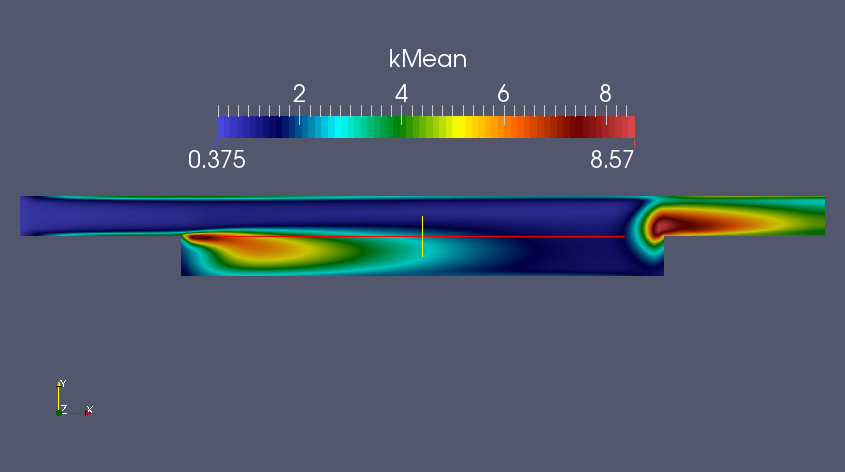
\includegraphics[width=0.95\linewidth]{simple_ko_10_mean_k.png}
	\end{subfigure}
	\begin{subfigure}{0.5\textwidth}
		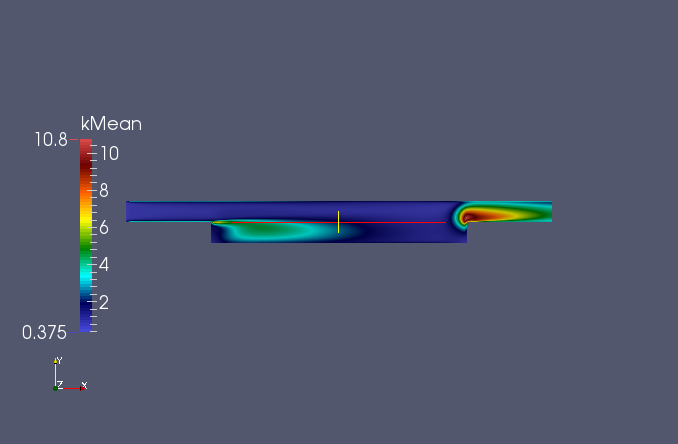
\includegraphics[width=0.95\linewidth]{simple_ko_20_mean_k.png}
	\end{subfigure}
\end{figure}
\\
\section*{4)}
\section*{5)}
\section*{6)}
Since turbulence is a three-dimensional phenomenon, I would assume that some critical information could be lost using LES as a 2D model. One example could be an eddy with primarily extension in the z-direction, that might have a width below the cutoff value in the x- or y-directions. Thus the impact of this eddy on the mean flow, which might be significant, could potentially be lost by using only a 2D approach.
 \end{document}
